%% prisma_flow.tex — PRISMA-ScR Flowchart
%% Included via %% prisma_flow.tex — PRISMA-ScR Flowchart
%% Included via %% prisma_flow.tex — PRISMA-ScR Flowchart
%% Included via %% prisma_flow.tex — PRISMA-ScR Flowchart
%% Included via \input{prisma_flow} in the figure environment of main.tex
%% Exact counts: 5,621 identified across 5 databases, 2,432 duplicates removed,
%% 3,189 screened by title (2,680 excluded), 509 screened by abstract
%% (474 excluded), 35 full text (databases) + 7 snowballing, 18 excluded,
%% 24 included (17 databases + 7 snowballing).

\usetikzlibrary{positioning, calc, arrows.meta}

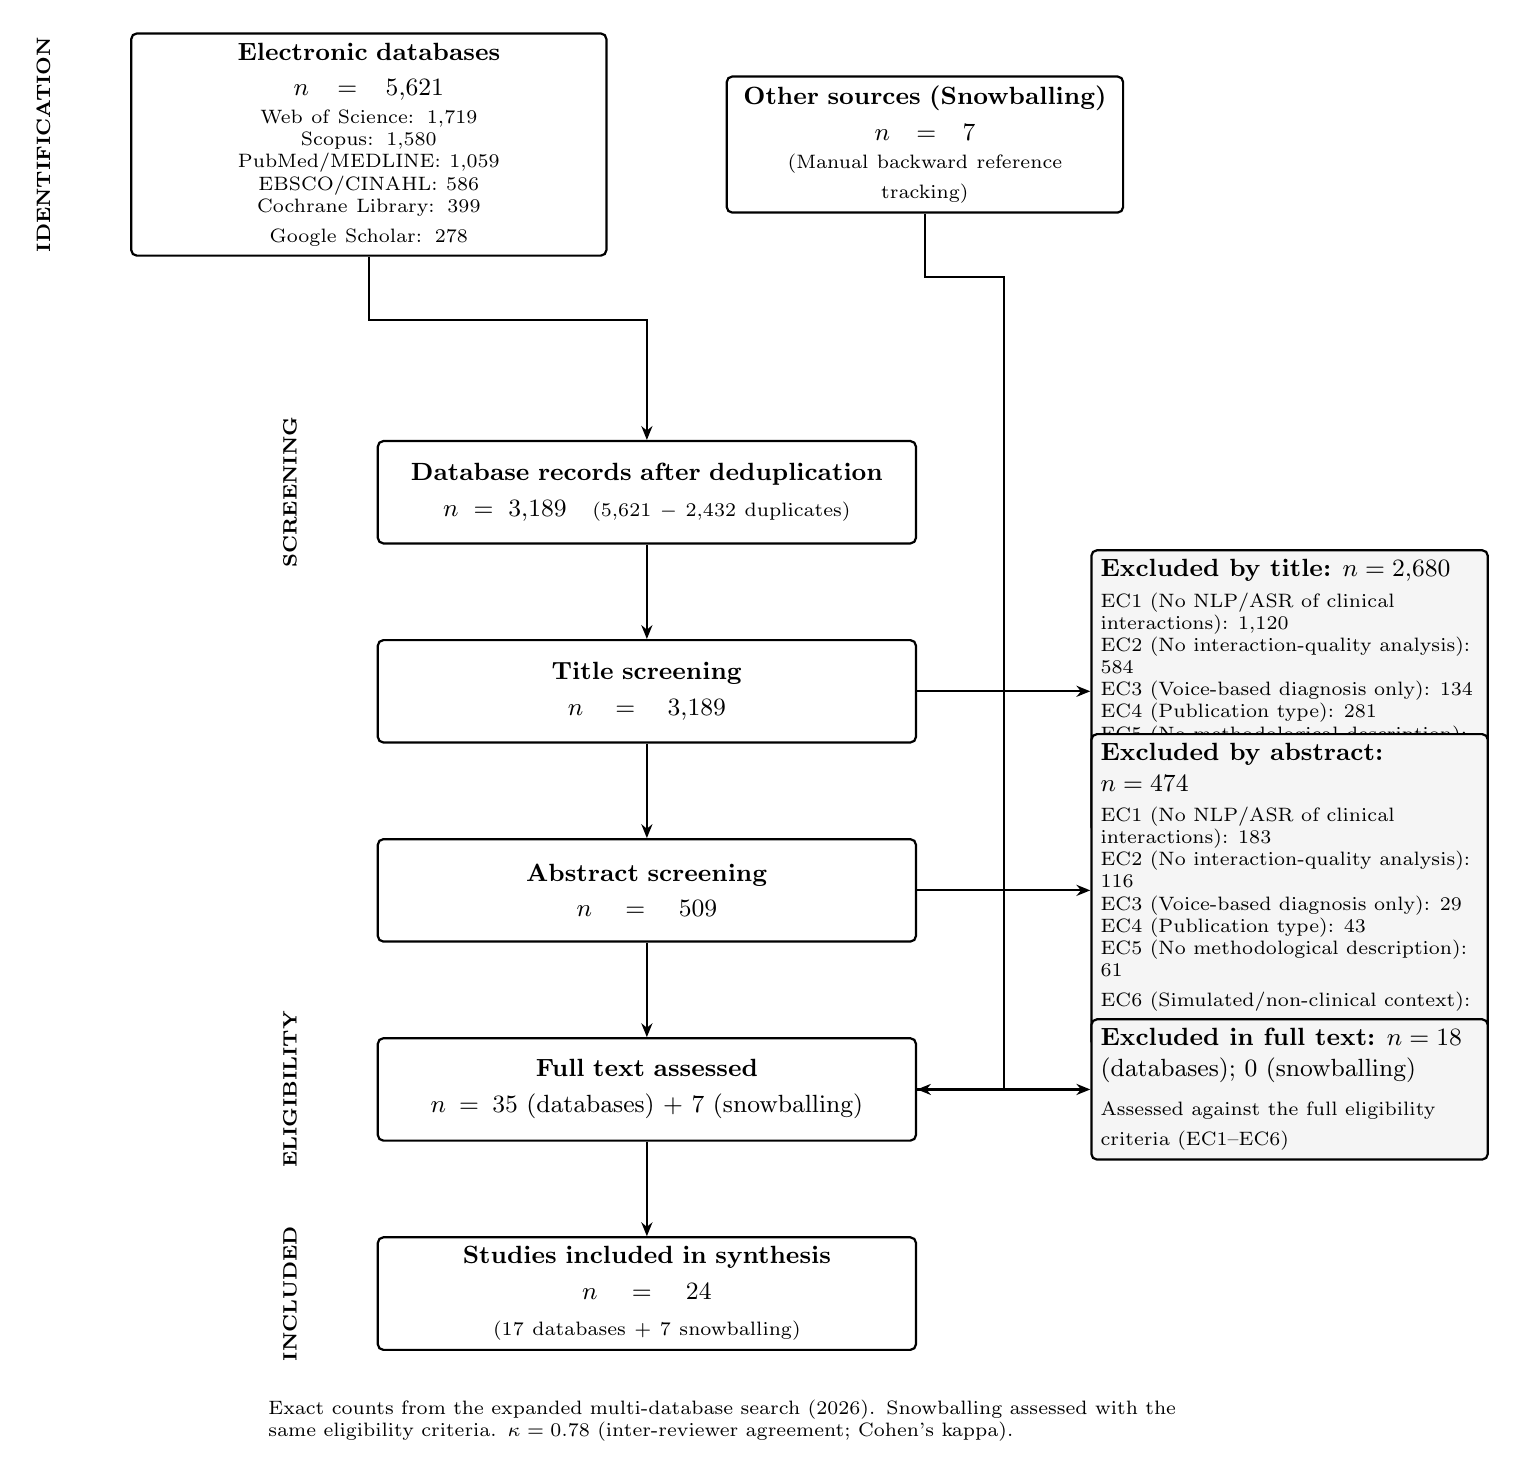
\begin{tikzpicture}[
  %% main flow boxes
  mbox/.style={
    rectangle, draw=black, thick, rounded corners=2pt,
    minimum width=6.8cm, text width=6.6cm,
    minimum height=1.3cm, align=center,
    fill=white, font=\small
  },
  %% exclusion boxes (right margin)
  ebox/.style={
    rectangle, draw=black, thick, rounded corners=2pt,
    minimum width=5.0cm, text width=4.8cm,
    minimum height=1.3cm, align=flush left,
    fill=gray!8, font=\small
  },
  %% arrows
  arr/.style={-{Stealth[length=5pt,width=4pt]}, thick},
  %% phase labels
  phase/.style={font=\bfseries\scriptsize, rotate=90, anchor=center}
]

%% ================================================================
%% PHASE 1 — IDENTIFICATION
%% ================================================================
\node[mbox, minimum width=6.0cm, text width=5.8cm] (dbbox) at (-1.8, 0) {
  \textbf{Electronic databases}\\[2pt]
  $n = 5{,}621$\\[2pt]
  {\scriptsize Web of Science: 1,719\\
    Scopus: 1,580\\
    PubMed/MEDLINE: 1,059\\
    EBSCO/CINAHL: 586\\
    Cochrane Library: 399\\
    Google Scholar: 278}
};

\node[mbox, minimum width=5.0cm, text width=4.8cm,
      right=1.5cm of dbbox] (otherbox) {
  \textbf{Other sources (Snowballing)}\\[2pt]
  $n = 7$\\[2pt]
  {\scriptsize (Manual backward reference\\
    tracking)}
};

%% ================================================================
%% PHASE 2 — SCREENING
%% ================================================================
\coordinate (midid) at ($(dbbox.south)!0.5!(otherbox.south)$);

\node[mbox, below=2.6cm of midid, anchor=north] (dedup) {
  \textbf{Database records after deduplication}\\[2pt]
  $n = 3{,}189$\quad{\scriptsize (5,621 $-$ 2,432 duplicates)}
};

%% arrow from databases to deduplication
\draw[arr] (dbbox.south) -- ++(0,-0.8cm) -| (dedup.north);

\node[mbox, below=1.2cm of dedup] (screen1) {
  \textbf{Title screening}\\[2pt]
  $n = 3{,}189$
};

\draw[arr] (dedup) -- (screen1);

\node[ebox, right=2.2cm of screen1] (excl1) {
  \textbf{Excluded by title:} $n = 2{,}680$\\[3pt]
  {\scriptsize
    EC1 (No NLP/ASR of clinical interactions): 1,120\\
    EC2 (No interaction-quality analysis): 584\\
    EC3 (Voice-based diagnosis only): 134\\
    EC4 (Publication type): 281\\
    EC5 (No methodological description): 358\\
    EC6 (Simulated/non-clinical context): 203
  }
};

\draw[arr] (screen1.east) -- (excl1.west);

\node[mbox, below=1.2cm of screen1] (screen2) {
  \textbf{Abstract screening}\\[2pt]
  $n = 509$
};

\draw[arr] (screen1) -- (screen2);

\node[ebox, right=2.2cm of screen2] (excl2) {
  \textbf{Excluded by abstract:} $n = 474$\\[3pt]
  {\scriptsize
    EC1 (No NLP/ASR of clinical interactions): 183\\
    EC2 (No interaction-quality analysis): 116\\
    EC3 (Voice-based diagnosis only): 29\\
    EC4 (Publication type): 43\\
    EC5 (No methodological description): 61\\
    EC6 (Simulated/non-clinical context): 42
  }
};

\draw[arr] (screen2.east) -- (excl2.west);

%% ================================================================
%% PHASE 3 — ELIGIBILITY
%% ================================================================
\node[mbox, below=1.2cm of screen2] (eligib) {
  \textbf{Full text assessed}\\[2pt]
  $n = 35$ (databases) $+$ $7$ (snowballing)
};

\draw[arr] (screen2) -- (eligib);

%% snowballing enters directly at eligibility (bypasses screening)
\draw[arr] (otherbox.south) -- ++(0,-0.8cm) -| ([xshift=1.1cm]eligib.east) -- (eligib.east);

\node[ebox, right=2.2cm of eligib] (excl3) {
  \textbf{Excluded in full text:} $n = 18$ (databases); $0$ (snowballing)\\[3pt]
  {\scriptsize
    Assessed against the full eligibility criteria (EC1--EC6)
  }
};

\draw[arr] (eligib.east) -- (excl3.west);

%% ================================================================
%% PHASE 4 — INCLUDED
%% ================================================================
\node[mbox, below=1.2cm of eligib] (included) {
  \textbf{Studies included in synthesis}\\[2pt]
  $n = 24$\\[2pt]
  {\scriptsize (17 databases + 7 snowballing)}
};

\draw[arr] (eligib) -- (included);

%% ================================================================
%% PHASE LABELS (left margin)
%% ================================================================
\node[phase] at ($(dbbox.west) + (-1.1cm, 0)$)      {IDENTIFICATION};
\node[phase] at ($(dedup.west)  + (-1.1cm, 0)$)      {SCREENING};
\node[phase] at ($(screen1.west) + (-1.1cm, 0)$)      {};   %% screening continues
\node[phase] at ($(screen2.west) + (-1.1cm, 0)$)      {};   %% screening continues
\node[phase] at ($(eligib.west) + (-1.1cm, 0)$)      {ELIGIBILITY};
\node[phase] at ($(included.west) + (-1.1cm, 0)$)    {INCLUDED};

%% ================================================================
%% FOOTNOTE
%% ================================================================
\node[font=\scriptsize, anchor=north west, text width=12cm]
  at ($(included.south west) + (-1.5cm, -0.5cm)$) {%
  Exact counts from the expanded multi-database search (2026).
  Snowballing assessed with the same eligibility criteria.
  $\kappa = 0.78$ (inter-reviewer agreement; Cohen's kappa).
};

\end{tikzpicture}
 in the figure environment of main.tex
%% Exact counts: 5,621 identified across 5 databases, 2,432 duplicates removed,
%% 3,189 screened by title (2,680 excluded), 509 screened by abstract
%% (474 excluded), 35 full text (databases) + 7 snowballing, 18 excluded,
%% 24 included (17 databases + 7 snowballing).

\usetikzlibrary{positioning, calc, arrows.meta}

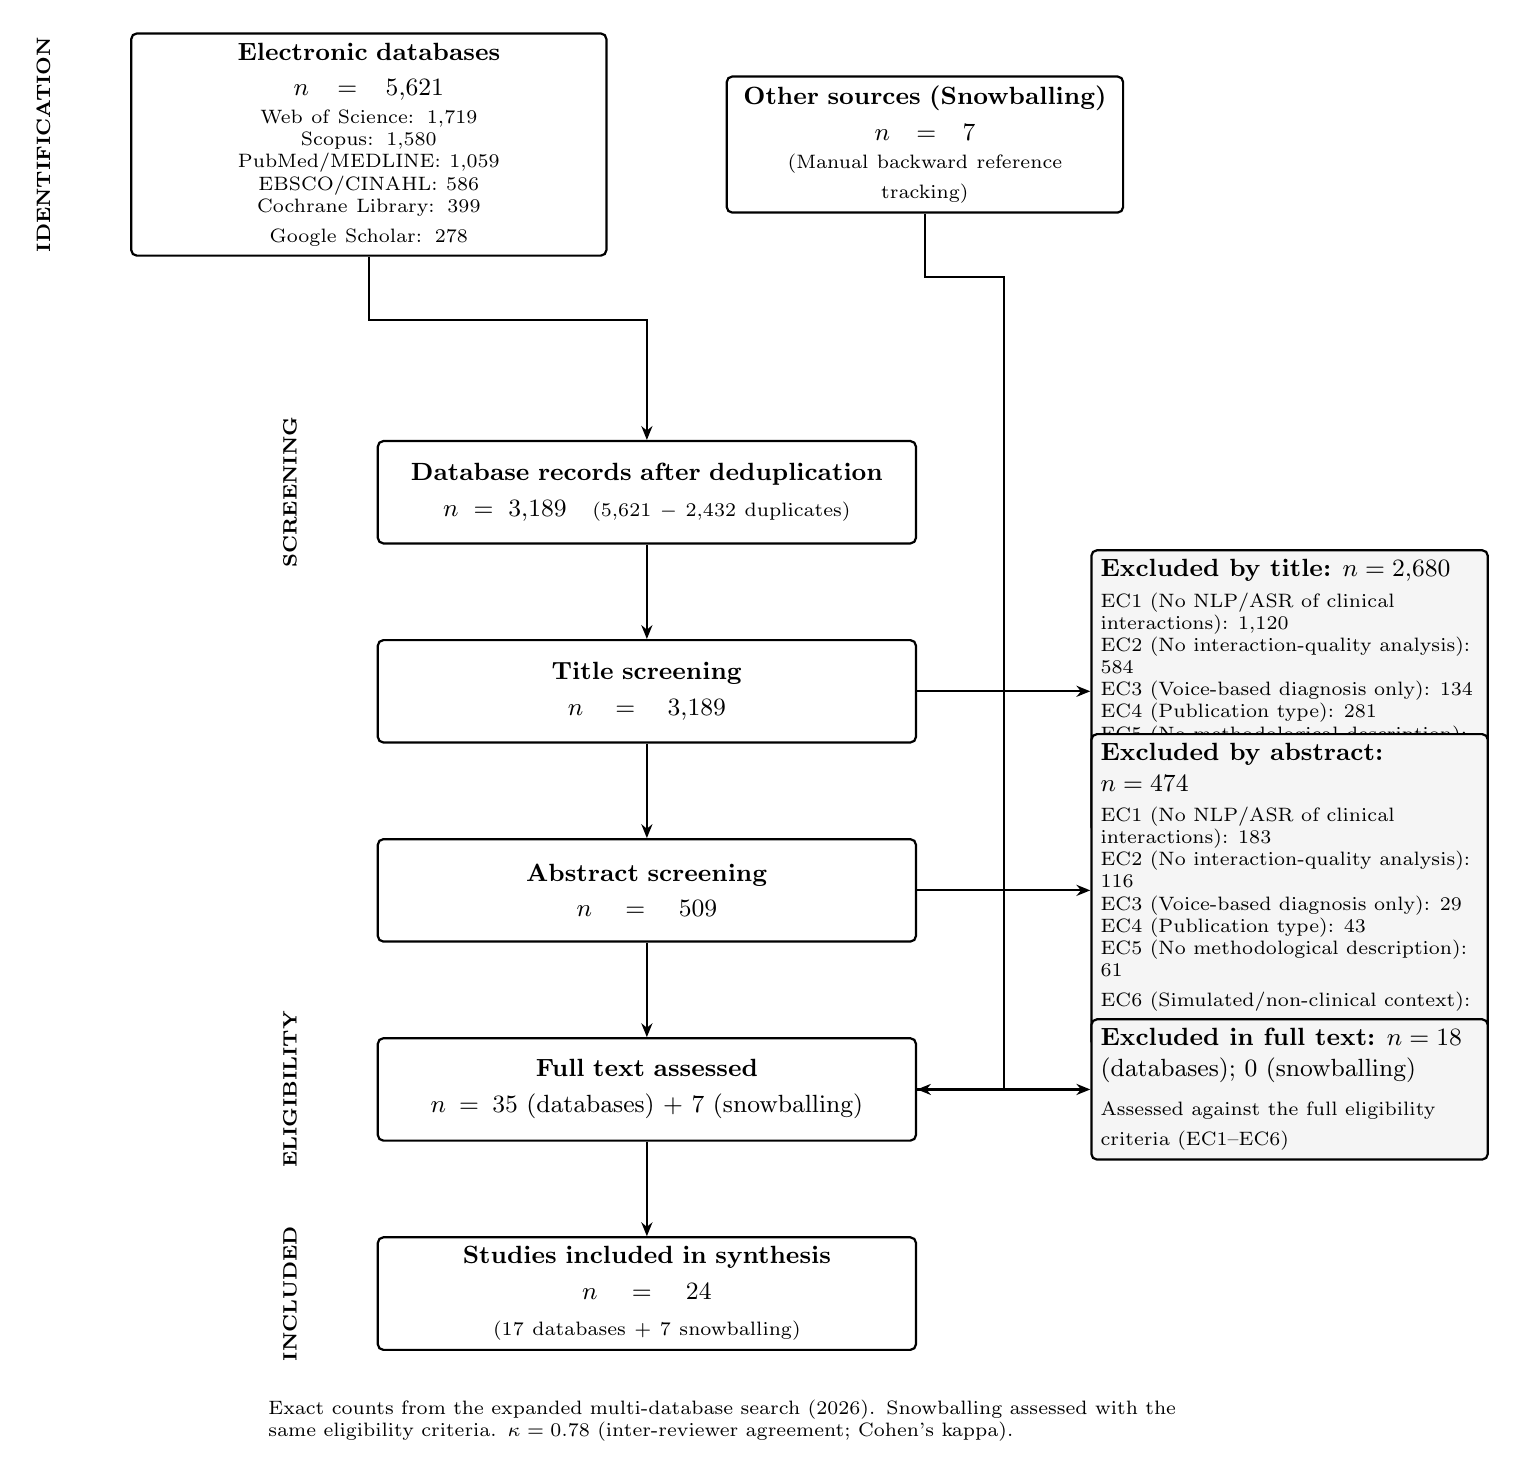
\begin{tikzpicture}[
  %% main flow boxes
  mbox/.style={
    rectangle, draw=black, thick, rounded corners=2pt,
    minimum width=6.8cm, text width=6.6cm,
    minimum height=1.3cm, align=center,
    fill=white, font=\small
  },
  %% exclusion boxes (right margin)
  ebox/.style={
    rectangle, draw=black, thick, rounded corners=2pt,
    minimum width=5.0cm, text width=4.8cm,
    minimum height=1.3cm, align=flush left,
    fill=gray!8, font=\small
  },
  %% arrows
  arr/.style={-{Stealth[length=5pt,width=4pt]}, thick},
  %% phase labels
  phase/.style={font=\bfseries\scriptsize, rotate=90, anchor=center}
]

%% ================================================================
%% PHASE 1 — IDENTIFICATION
%% ================================================================
\node[mbox, minimum width=6.0cm, text width=5.8cm] (dbbox) at (-1.8, 0) {
  \textbf{Electronic databases}\\[2pt]
  $n = 5{,}621$\\[2pt]
  {\scriptsize Web of Science: 1,719\\
    Scopus: 1,580\\
    PubMed/MEDLINE: 1,059\\
    EBSCO/CINAHL: 586\\
    Cochrane Library: 399\\
    Google Scholar: 278}
};

\node[mbox, minimum width=5.0cm, text width=4.8cm,
      right=1.5cm of dbbox] (otherbox) {
  \textbf{Other sources (Snowballing)}\\[2pt]
  $n = 7$\\[2pt]
  {\scriptsize (Manual backward reference\\
    tracking)}
};

%% ================================================================
%% PHASE 2 — SCREENING
%% ================================================================
\coordinate (midid) at ($(dbbox.south)!0.5!(otherbox.south)$);

\node[mbox, below=2.6cm of midid, anchor=north] (dedup) {
  \textbf{Database records after deduplication}\\[2pt]
  $n = 3{,}189$\quad{\scriptsize (5,621 $-$ 2,432 duplicates)}
};

%% arrow from databases to deduplication
\draw[arr] (dbbox.south) -- ++(0,-0.8cm) -| (dedup.north);

\node[mbox, below=1.2cm of dedup] (screen1) {
  \textbf{Title screening}\\[2pt]
  $n = 3{,}189$
};

\draw[arr] (dedup) -- (screen1);

\node[ebox, right=2.2cm of screen1] (excl1) {
  \textbf{Excluded by title:} $n = 2{,}680$\\[3pt]
  {\scriptsize
    EC1 (No NLP/ASR of clinical interactions): 1,120\\
    EC2 (No interaction-quality analysis): 584\\
    EC3 (Voice-based diagnosis only): 134\\
    EC4 (Publication type): 281\\
    EC5 (No methodological description): 358\\
    EC6 (Simulated/non-clinical context): 203
  }
};

\draw[arr] (screen1.east) -- (excl1.west);

\node[mbox, below=1.2cm of screen1] (screen2) {
  \textbf{Abstract screening}\\[2pt]
  $n = 509$
};

\draw[arr] (screen1) -- (screen2);

\node[ebox, right=2.2cm of screen2] (excl2) {
  \textbf{Excluded by abstract:} $n = 474$\\[3pt]
  {\scriptsize
    EC1 (No NLP/ASR of clinical interactions): 183\\
    EC2 (No interaction-quality analysis): 116\\
    EC3 (Voice-based diagnosis only): 29\\
    EC4 (Publication type): 43\\
    EC5 (No methodological description): 61\\
    EC6 (Simulated/non-clinical context): 42
  }
};

\draw[arr] (screen2.east) -- (excl2.west);

%% ================================================================
%% PHASE 3 — ELIGIBILITY
%% ================================================================
\node[mbox, below=1.2cm of screen2] (eligib) {
  \textbf{Full text assessed}\\[2pt]
  $n = 35$ (databases) $+$ $7$ (snowballing)
};

\draw[arr] (screen2) -- (eligib);

%% snowballing enters directly at eligibility (bypasses screening)
\draw[arr] (otherbox.south) -- ++(0,-0.8cm) -| ([xshift=1.1cm]eligib.east) -- (eligib.east);

\node[ebox, right=2.2cm of eligib] (excl3) {
  \textbf{Excluded in full text:} $n = 18$ (databases); $0$ (snowballing)\\[3pt]
  {\scriptsize
    Assessed against the full eligibility criteria (EC1--EC6)
  }
};

\draw[arr] (eligib.east) -- (excl3.west);

%% ================================================================
%% PHASE 4 — INCLUDED
%% ================================================================
\node[mbox, below=1.2cm of eligib] (included) {
  \textbf{Studies included in synthesis}\\[2pt]
  $n = 24$\\[2pt]
  {\scriptsize (17 databases + 7 snowballing)}
};

\draw[arr] (eligib) -- (included);

%% ================================================================
%% PHASE LABELS (left margin)
%% ================================================================
\node[phase] at ($(dbbox.west) + (-1.1cm, 0)$)      {IDENTIFICATION};
\node[phase] at ($(dedup.west)  + (-1.1cm, 0)$)      {SCREENING};
\node[phase] at ($(screen1.west) + (-1.1cm, 0)$)      {};   %% screening continues
\node[phase] at ($(screen2.west) + (-1.1cm, 0)$)      {};   %% screening continues
\node[phase] at ($(eligib.west) + (-1.1cm, 0)$)      {ELIGIBILITY};
\node[phase] at ($(included.west) + (-1.1cm, 0)$)    {INCLUDED};

%% ================================================================
%% FOOTNOTE
%% ================================================================
\node[font=\scriptsize, anchor=north west, text width=12cm]
  at ($(included.south west) + (-1.5cm, -0.5cm)$) {%
  Exact counts from the expanded multi-database search (2026).
  Snowballing assessed with the same eligibility criteria.
  $\kappa = 0.78$ (inter-reviewer agreement; Cohen's kappa).
};

\end{tikzpicture}
 in the figure environment of main.tex
%% Exact counts: 5,621 identified across 5 databases, 2,432 duplicates removed,
%% 3,189 screened by title (2,680 excluded), 509 screened by abstract
%% (474 excluded), 35 full text (databases) + 7 snowballing, 18 excluded,
%% 24 included (17 databases + 7 snowballing).

\usetikzlibrary{positioning, calc, arrows.meta}

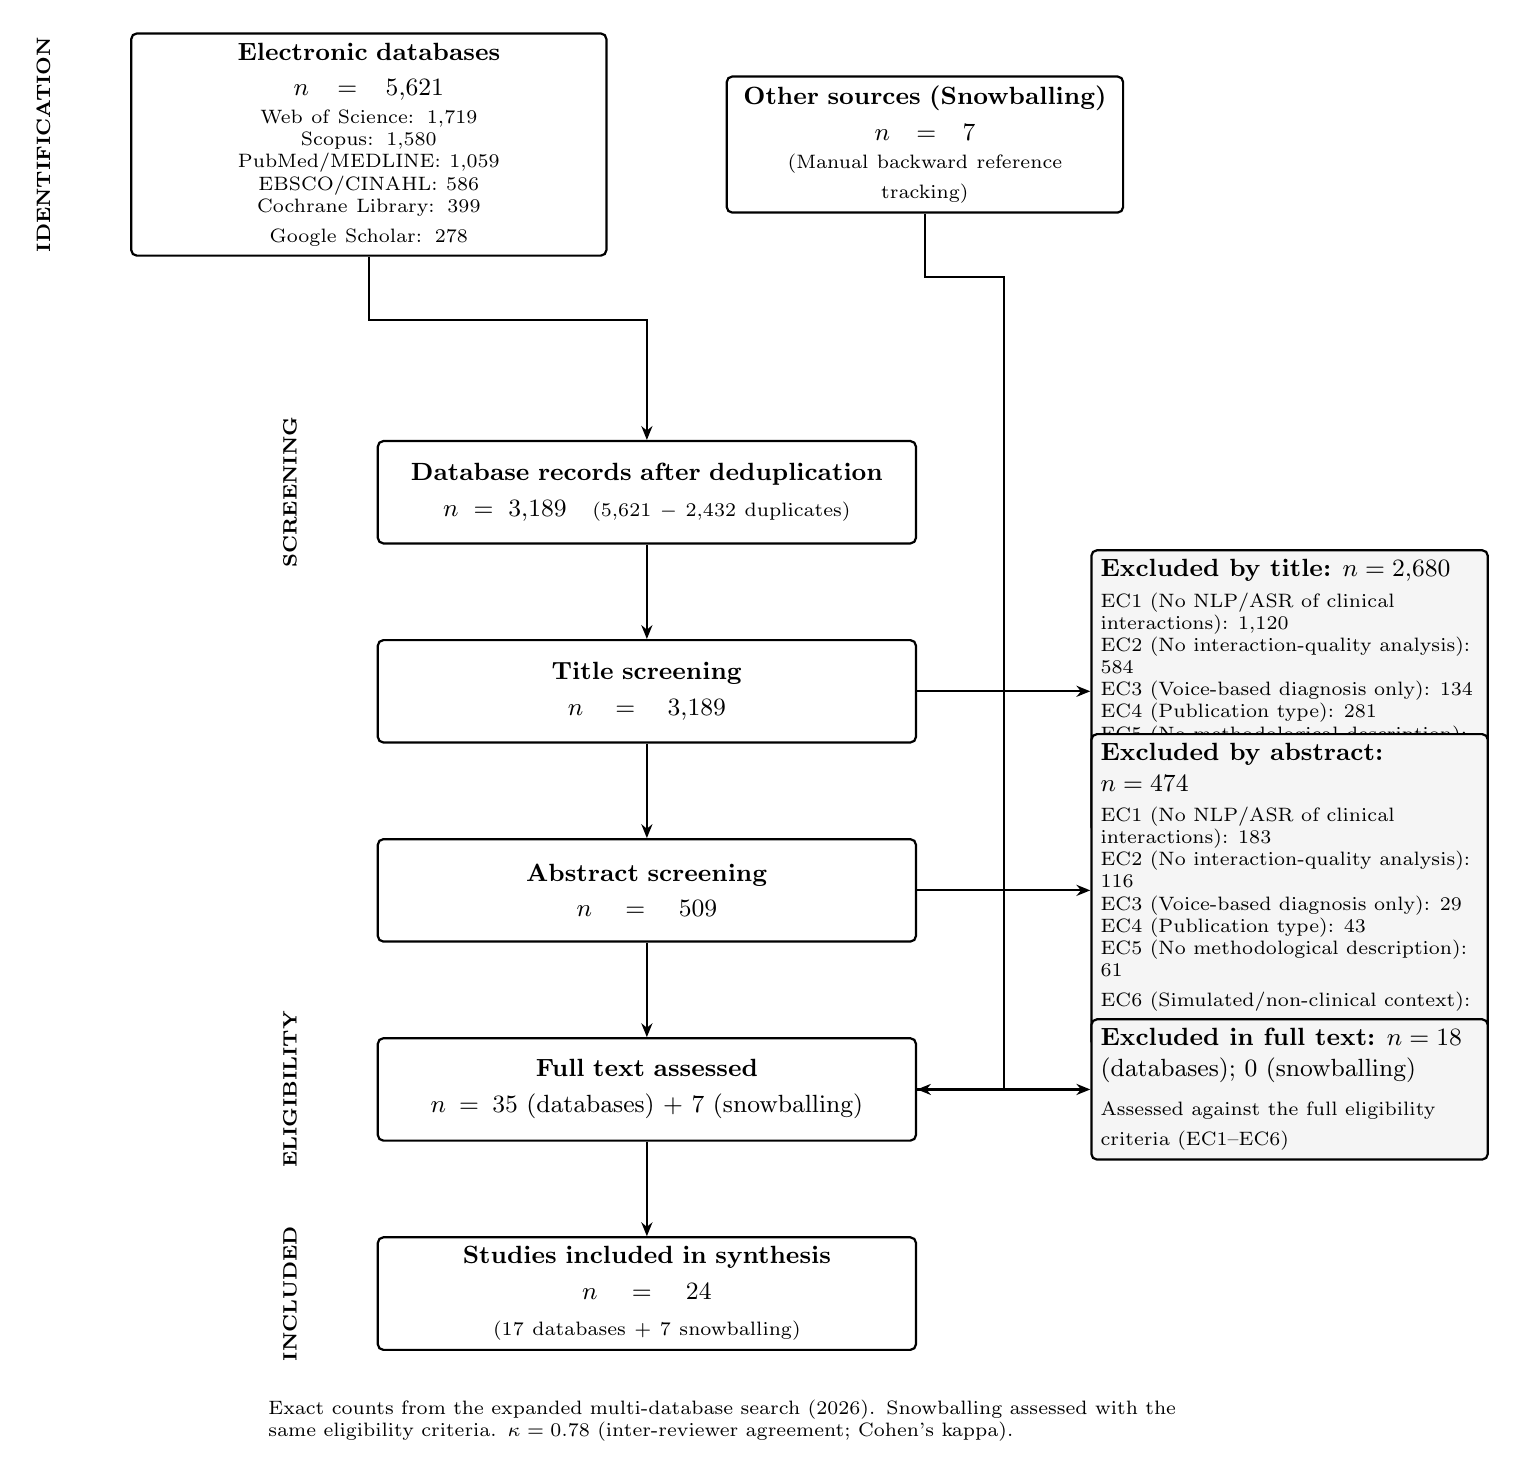
\begin{tikzpicture}[
  %% main flow boxes
  mbox/.style={
    rectangle, draw=black, thick, rounded corners=2pt,
    minimum width=6.8cm, text width=6.6cm,
    minimum height=1.3cm, align=center,
    fill=white, font=\small
  },
  %% exclusion boxes (right margin)
  ebox/.style={
    rectangle, draw=black, thick, rounded corners=2pt,
    minimum width=5.0cm, text width=4.8cm,
    minimum height=1.3cm, align=flush left,
    fill=gray!8, font=\small
  },
  %% arrows
  arr/.style={-{Stealth[length=5pt,width=4pt]}, thick},
  %% phase labels
  phase/.style={font=\bfseries\scriptsize, rotate=90, anchor=center}
]

%% ================================================================
%% PHASE 1 — IDENTIFICATION
%% ================================================================
\node[mbox, minimum width=6.0cm, text width=5.8cm] (dbbox) at (-1.8, 0) {
  \textbf{Electronic databases}\\[2pt]
  $n = 5{,}621$\\[2pt]
  {\scriptsize Web of Science: 1,719\\
    Scopus: 1,580\\
    PubMed/MEDLINE: 1,059\\
    EBSCO/CINAHL: 586\\
    Cochrane Library: 399\\
    Google Scholar: 278}
};

\node[mbox, minimum width=5.0cm, text width=4.8cm,
      right=1.5cm of dbbox] (otherbox) {
  \textbf{Other sources (Snowballing)}\\[2pt]
  $n = 7$\\[2pt]
  {\scriptsize (Manual backward reference\\
    tracking)}
};

%% ================================================================
%% PHASE 2 — SCREENING
%% ================================================================
\coordinate (midid) at ($(dbbox.south)!0.5!(otherbox.south)$);

\node[mbox, below=2.6cm of midid, anchor=north] (dedup) {
  \textbf{Database records after deduplication}\\[2pt]
  $n = 3{,}189$\quad{\scriptsize (5,621 $-$ 2,432 duplicates)}
};

%% arrow from databases to deduplication
\draw[arr] (dbbox.south) -- ++(0,-0.8cm) -| (dedup.north);

\node[mbox, below=1.2cm of dedup] (screen1) {
  \textbf{Title screening}\\[2pt]
  $n = 3{,}189$
};

\draw[arr] (dedup) -- (screen1);

\node[ebox, right=2.2cm of screen1] (excl1) {
  \textbf{Excluded by title:} $n = 2{,}680$\\[3pt]
  {\scriptsize
    EC1 (No NLP/ASR of clinical interactions): 1,120\\
    EC2 (No interaction-quality analysis): 584\\
    EC3 (Voice-based diagnosis only): 134\\
    EC4 (Publication type): 281\\
    EC5 (No methodological description): 358\\
    EC6 (Simulated/non-clinical context): 203
  }
};

\draw[arr] (screen1.east) -- (excl1.west);

\node[mbox, below=1.2cm of screen1] (screen2) {
  \textbf{Abstract screening}\\[2pt]
  $n = 509$
};

\draw[arr] (screen1) -- (screen2);

\node[ebox, right=2.2cm of screen2] (excl2) {
  \textbf{Excluded by abstract:} $n = 474$\\[3pt]
  {\scriptsize
    EC1 (No NLP/ASR of clinical interactions): 183\\
    EC2 (No interaction-quality analysis): 116\\
    EC3 (Voice-based diagnosis only): 29\\
    EC4 (Publication type): 43\\
    EC5 (No methodological description): 61\\
    EC6 (Simulated/non-clinical context): 42
  }
};

\draw[arr] (screen2.east) -- (excl2.west);

%% ================================================================
%% PHASE 3 — ELIGIBILITY
%% ================================================================
\node[mbox, below=1.2cm of screen2] (eligib) {
  \textbf{Full text assessed}\\[2pt]
  $n = 35$ (databases) $+$ $7$ (snowballing)
};

\draw[arr] (screen2) -- (eligib);

%% snowballing enters directly at eligibility (bypasses screening)
\draw[arr] (otherbox.south) -- ++(0,-0.8cm) -| ([xshift=1.1cm]eligib.east) -- (eligib.east);

\node[ebox, right=2.2cm of eligib] (excl3) {
  \textbf{Excluded in full text:} $n = 18$ (databases); $0$ (snowballing)\\[3pt]
  {\scriptsize
    Assessed against the full eligibility criteria (EC1--EC6)
  }
};

\draw[arr] (eligib.east) -- (excl3.west);

%% ================================================================
%% PHASE 4 — INCLUDED
%% ================================================================
\node[mbox, below=1.2cm of eligib] (included) {
  \textbf{Studies included in synthesis}\\[2pt]
  $n = 24$\\[2pt]
  {\scriptsize (17 databases + 7 snowballing)}
};

\draw[arr] (eligib) -- (included);

%% ================================================================
%% PHASE LABELS (left margin)
%% ================================================================
\node[phase] at ($(dbbox.west) + (-1.1cm, 0)$)      {IDENTIFICATION};
\node[phase] at ($(dedup.west)  + (-1.1cm, 0)$)      {SCREENING};
\node[phase] at ($(screen1.west) + (-1.1cm, 0)$)      {};   %% screening continues
\node[phase] at ($(screen2.west) + (-1.1cm, 0)$)      {};   %% screening continues
\node[phase] at ($(eligib.west) + (-1.1cm, 0)$)      {ELIGIBILITY};
\node[phase] at ($(included.west) + (-1.1cm, 0)$)    {INCLUDED};

%% ================================================================
%% FOOTNOTE
%% ================================================================
\node[font=\scriptsize, anchor=north west, text width=12cm]
  at ($(included.south west) + (-1.5cm, -0.5cm)$) {%
  Exact counts from the expanded multi-database search (2026).
  Snowballing assessed with the same eligibility criteria.
  $\kappa = 0.78$ (inter-reviewer agreement; Cohen's kappa).
};

\end{tikzpicture}
 in the figure environment of main.tex
%% Exact counts: 5,621 identified across 5 databases, 2,432 duplicates removed,
%% 3,189 screened by title (2,680 excluded), 509 screened by abstract
%% (474 excluded), 35 full text (databases) + 7 snowballing, 18 excluded,
%% 24 included (17 databases + 7 snowballing).

\usetikzlibrary{positioning, calc, arrows.meta}

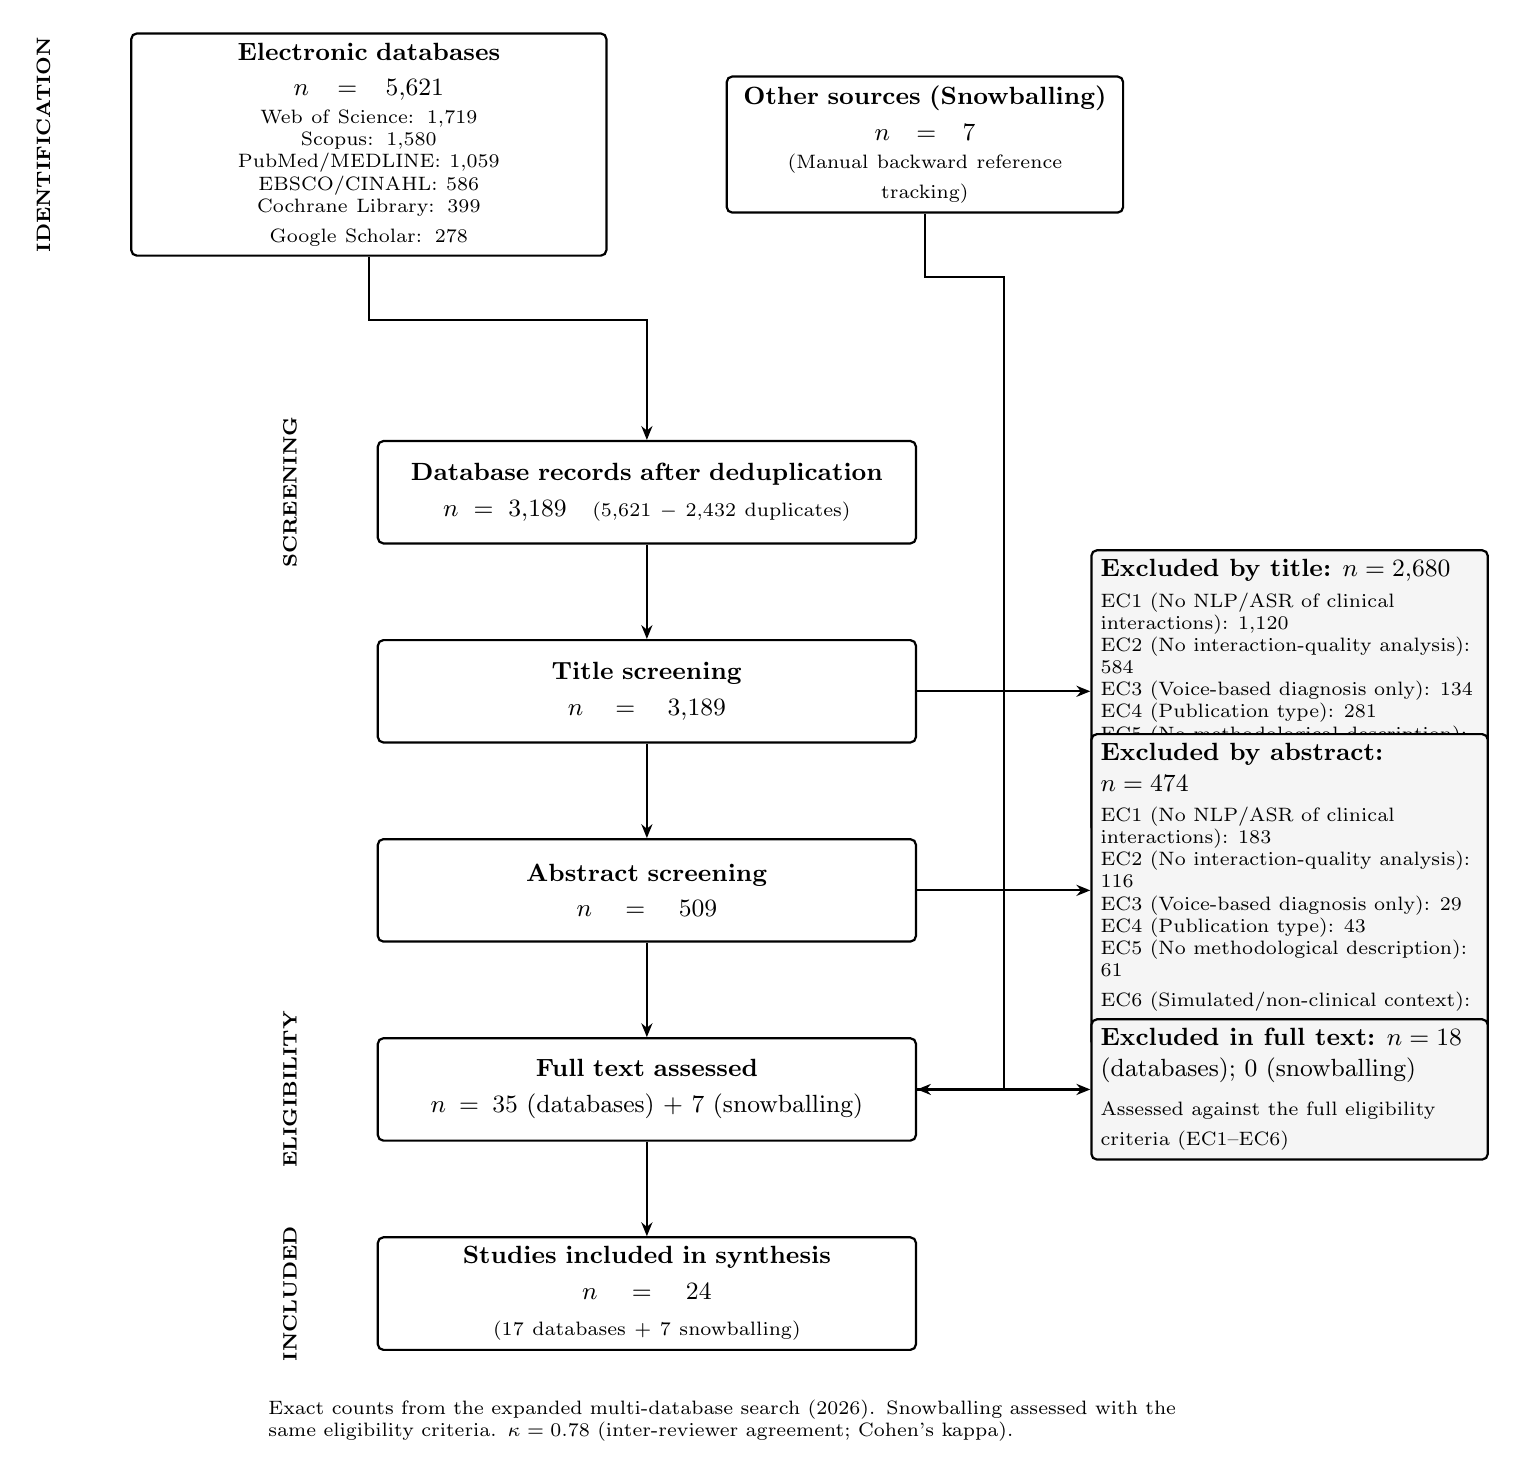
\begin{tikzpicture}[
  %% main flow boxes
  mbox/.style={
    rectangle, draw=black, thick, rounded corners=2pt,
    minimum width=6.8cm, text width=6.6cm,
    minimum height=1.3cm, align=center,
    fill=white, font=\small
  },
  %% exclusion boxes (right margin)
  ebox/.style={
    rectangle, draw=black, thick, rounded corners=2pt,
    minimum width=5.0cm, text width=4.8cm,
    minimum height=1.3cm, align=flush left,
    fill=gray!8, font=\small
  },
  %% arrows
  arr/.style={-{Stealth[length=5pt,width=4pt]}, thick},
  %% phase labels
  phase/.style={font=\bfseries\scriptsize, rotate=90, anchor=center}
]

%% ================================================================
%% PHASE 1 — IDENTIFICATION
%% ================================================================
\node[mbox, minimum width=6.0cm, text width=5.8cm] (dbbox) at (-1.8, 0) {
  \textbf{Electronic databases}\\[2pt]
  $n = 5{,}621$\\[2pt]
  {\scriptsize Web of Science: 1,719\\
    Scopus: 1,580\\
    PubMed/MEDLINE: 1,059\\
    EBSCO/CINAHL: 586\\
    Cochrane Library: 399\\
    Google Scholar: 278}
};

\node[mbox, minimum width=5.0cm, text width=4.8cm,
      right=1.5cm of dbbox] (otherbox) {
  \textbf{Other sources (Snowballing)}\\[2pt]
  $n = 7$\\[2pt]
  {\scriptsize (Manual backward reference\\
    tracking)}
};

%% ================================================================
%% PHASE 2 — SCREENING
%% ================================================================
\coordinate (midid) at ($(dbbox.south)!0.5!(otherbox.south)$);

\node[mbox, below=2.6cm of midid, anchor=north] (dedup) {
  \textbf{Database records after deduplication}\\[2pt]
  $n = 3{,}189$\quad{\scriptsize (5,621 $-$ 2,432 duplicates)}
};

%% arrow from databases to deduplication
\draw[arr] (dbbox.south) -- ++(0,-0.8cm) -| (dedup.north);

\node[mbox, below=1.2cm of dedup] (screen1) {
  \textbf{Title screening}\\[2pt]
  $n = 3{,}189$
};

\draw[arr] (dedup) -- (screen1);

\node[ebox, right=2.2cm of screen1] (excl1) {
  \textbf{Excluded by title:} $n = 2{,}680$\\[3pt]
  {\scriptsize
    EC1 (No NLP/ASR of clinical interactions): 1,120\\
    EC2 (No interaction-quality analysis): 584\\
    EC3 (Voice-based diagnosis only): 134\\
    EC4 (Publication type): 281\\
    EC5 (No methodological description): 358\\
    EC6 (Simulated/non-clinical context): 203
  }
};

\draw[arr] (screen1.east) -- (excl1.west);

\node[mbox, below=1.2cm of screen1] (screen2) {
  \textbf{Abstract screening}\\[2pt]
  $n = 509$
};

\draw[arr] (screen1) -- (screen2);

\node[ebox, right=2.2cm of screen2] (excl2) {
  \textbf{Excluded by abstract:} $n = 474$\\[3pt]
  {\scriptsize
    EC1 (No NLP/ASR of clinical interactions): 183\\
    EC2 (No interaction-quality analysis): 116\\
    EC3 (Voice-based diagnosis only): 29\\
    EC4 (Publication type): 43\\
    EC5 (No methodological description): 61\\
    EC6 (Simulated/non-clinical context): 42
  }
};

\draw[arr] (screen2.east) -- (excl2.west);

%% ================================================================
%% PHASE 3 — ELIGIBILITY
%% ================================================================
\node[mbox, below=1.2cm of screen2] (eligib) {
  \textbf{Full text assessed}\\[2pt]
  $n = 35$ (databases) $+$ $7$ (snowballing)
};

\draw[arr] (screen2) -- (eligib);

%% snowballing enters directly at eligibility (bypasses screening)
\draw[arr] (otherbox.south) -- ++(0,-0.8cm) -| ([xshift=1.1cm]eligib.east) -- (eligib.east);

\node[ebox, right=2.2cm of eligib] (excl3) {
  \textbf{Excluded in full text:} $n = 18$ (databases); $0$ (snowballing)\\[3pt]
  {\scriptsize
    Assessed against the full eligibility criteria (EC1--EC6)
  }
};

\draw[arr] (eligib.east) -- (excl3.west);

%% ================================================================
%% PHASE 4 — INCLUDED
%% ================================================================
\node[mbox, below=1.2cm of eligib] (included) {
  \textbf{Studies included in synthesis}\\[2pt]
  $n = 24$\\[2pt]
  {\scriptsize (17 databases + 7 snowballing)}
};

\draw[arr] (eligib) -- (included);

%% ================================================================
%% PHASE LABELS (left margin)
%% ================================================================
\node[phase] at ($(dbbox.west) + (-1.1cm, 0)$)      {IDENTIFICATION};
\node[phase] at ($(dedup.west)  + (-1.1cm, 0)$)      {SCREENING};
\node[phase] at ($(screen1.west) + (-1.1cm, 0)$)      {};   %% screening continues
\node[phase] at ($(screen2.west) + (-1.1cm, 0)$)      {};   %% screening continues
\node[phase] at ($(eligib.west) + (-1.1cm, 0)$)      {ELIGIBILITY};
\node[phase] at ($(included.west) + (-1.1cm, 0)$)    {INCLUDED};

%% ================================================================
%% FOOTNOTE
%% ================================================================
\node[font=\scriptsize, anchor=north west, text width=12cm]
  at ($(included.south west) + (-1.5cm, -0.5cm)$) {%
  Exact counts from the expanded multi-database search (2026).
  Snowballing assessed with the same eligibility criteria.
  $\kappa = 0.78$ (inter-reviewer agreement; Cohen's kappa).
};

\end{tikzpicture}
